\chapter{Metodología de Desarrollo y Planificación}
\label{cap:metodologiaDesarrollo}

En este capítulo se detalla la metodología de trabajo aplicada durante el proceso de desarrollo de la aplicación \textit{ClimbIt}. El objetivo principal ha sido establecer un flujo de trabajo con diversas herramientas de gestión, permitiendo avanzar de manera eficiente en las diferentes fases del proyecto. Además de esto, se desarrolla como el uso de metodológicas ágiles y herramientas de diseño ha facilitado la resolución de los problemas planteados de forma iterativa.

\section{Enfoque de Diseño Centrado en el Usuario (DCU)}

Tal como se expuso en los capítulos previos, la reciente popularización de la escalada ha provocado la entrada masiva de nuevos perfiles de deportistas con necesidades no cubiertas por las soluciones tecnológicas actuales. Ante esta situación, resultaba crucial que el proyecto adoptara desde su inicio un enfoque de Diseño Centrado en el Usuario (DCU) \citep{abras2004user}. El DCU es una filosofía de diseño que tiene por objeto la creación de productos que resuelvan necesidades concretas, situando a los usuarios finales en el centro de todas las fases de desarrollo e involucrándolos activamente.

Para garantizar el desarrollo de una solución que realmente aporte valor y reduzca las frustraciones actuales de los escaladores, las actividades de análisis y diseño  de requisitos se estructuraron de la siguiente manera:

\begin{enumerate}
\item \textbf{Empatía y conceptualización inicial:} Creación de un \textit{Value Proposition Canvas} (Lienzo de Propuesta de Valor del usuario) para modelar al usuario y definir la solución teórica.
\item \textbf{Definición del viaje del usuario y priorización:} Elaboración de un \textit{User Story Map} para estructurar las funcionalidades y acotar el Producto Mínimo Viable (MVP).
\item \textbf{Iteraciones y validación:} Realización de pruebas directas con usuarios reales para validar los requisitos capturados y testear las diferentes versiones 
(cuyos resultados se exponen detalladamente en el Capítulo \ref{cap:pruebasValidacion}).
\end{enumerate}

\section{Captura de Requisitos y Definición del Producto}

Antes de iniciar la fase de desarrollo e implementación, se determinó que era fundamental comprender en profundidad los problemas a resolver, evitando así el riesgo de basar el desarrollo en suposiciones no contrastadas. Por ello, apoyándonos en los fundamentos del DCU, se dedicó una fase inicial a la definición estratégica del producto mediante el uso de herramientas de diseño ágil.

\subsection{Lienzo de Propuesta de Valor (Value Proposition Canvas)}

Con el objetivo de empatizar de manera efectiva con el usuario final y ejecutar la primera tarea de diseño, se construyó un \textit{Value Proposition Canvas} (VPC), modelo propuesto por \cite{osterwalder2015value}. Esta herramienta permite situarse en la perspectiva del escalador y analizar su contexto dividiéndolo en dos bloques principales como se puede ver en la imagen \ref{fig:imagen_vpc}. A continaución se desarrollan cada uno de estos bloques:

\begin{figure}[h]
    \centering
    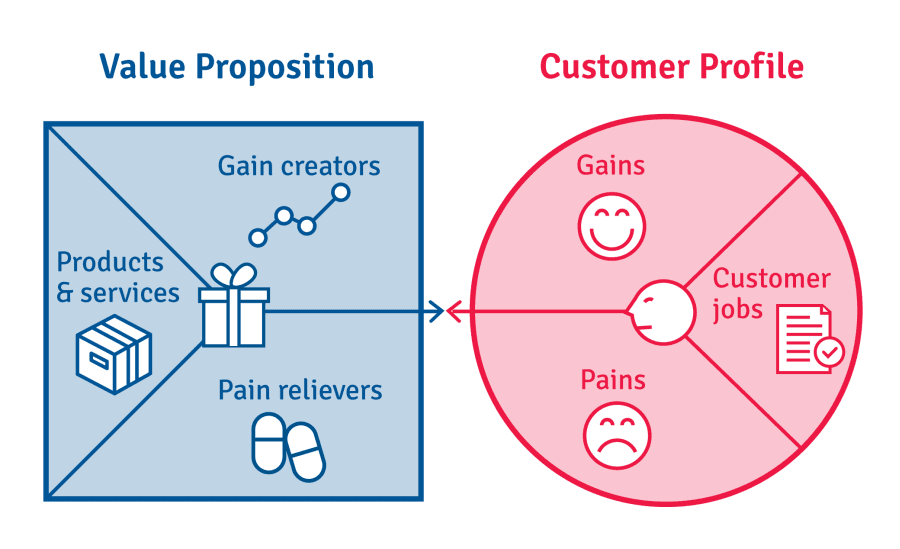
\includegraphics[width=0.8\textwidth]{./Imagenes/Fuentes/value-proposition-canvas.png} 
    \caption{Esquema de un Value Proposition Canvasi}
    \label{fig:imagen_vpc}
\end{figure}

\paragraph{Perfil del cliente:} 
Se enfoca exclusivamente en entender al usuario (en este caso el escalador). Se describen sus \textit{trabajos} (las tareas que intenta resolver), sus \textit{frustraciones} (los obstáculos y emociones negativas que encuentra) y sus \textit{ganancias} (los resultados y beneficios que desea obtener).Se determinó que el usuario escalador busca cumplir trabajos funcionales (registrar sesiones y visualizar progreso), sociales (compartir logros y competir en grupos) y emocionales (sentirse motivado) y que sus principales frustraciones giran en torno a la dificultad del registro manual, la falta de una plataforma centralizada y la desmotivación al no visualizar su progreso de manera clara.Por otro lado, sus ganancias deseadas son la facilidad para seguir su progreso, recibir retroalimentación constante y sentirse parte de una comunidad competitiva y sana.

\paragraph{Mapa de Valor:} 
Se centra en cómo un producto o servicio crea valor en base a los datos del perfil de cliente. Aquí se describen los \textit{aliviadores de frustraciones} (\textit{Pain Relievers}) y los \textit{creadores de ganancias} (\textit{Gain Creators}). Para dar respuesta al perfil analizado, se determinó que los \textit{Pain Relievers} de \textit{ClimbIt} debían ofrecer una interfaz altamente intuitiva, un registro simple del progreso y un entorno centralizado. Asimismo, sus \textit{Gain Creators} se apoyan en proporcionar estadísticas detalladas, un sistema de comparativa motivador y una competición social (sistema \textit{Leaderboards}) que impulse al usuario a mejorar e interactuar con su entorno.

\subsection{Visualización del viaje: User Story Map}

Basándose en la propuesta de valor, se realizo la construcción de un \textit{User Story Map} (USM), técnica definida por Jeff Patton, para visualizar el recorrido completo del usuario dentro de la aplicación \citep{patton2014user}, en este caso mediante la herramienta digital Mural. Un USM facilita la comprensión profunda del flujo de trabajo y las interacciones delusuario con el sistema, ayudando a visualizar y planificar las funcionalidades de manera global.

Este mapa visual resultó extremadamente útil a lo largo del desarollo del proyecto principalmente por el agrupamiento de los diferentes hitos, de manera que trazando líneas horizontales sobre el conjunto de historias agrupadas como se puede observar en la imagen \ref{fig:imagen_usm}. Se tomaron decisiones de diseño clave para decidir qué funcionalidades eran vitales para el primer prototip y cada uno de los diferentes hitos alcanzados permititendo dejar las ideas menos prioritarias para versiones futuras. Para visualizar en detalle el Mapa de Historia de Usuario de ClimbIt se puede hacer a través del siguiente enlace 
\footnote{Mapa de Historia de Usuario de ClimbIt: \url{https://app.mural.co/t/cm4232/m/cm4232/1719575921327/bb32e73a637ba77298937e8268d651afbee035e2?sender=u9565d89e69e5dee32c568362}}.

\begin{figure}[h]
    \centering
    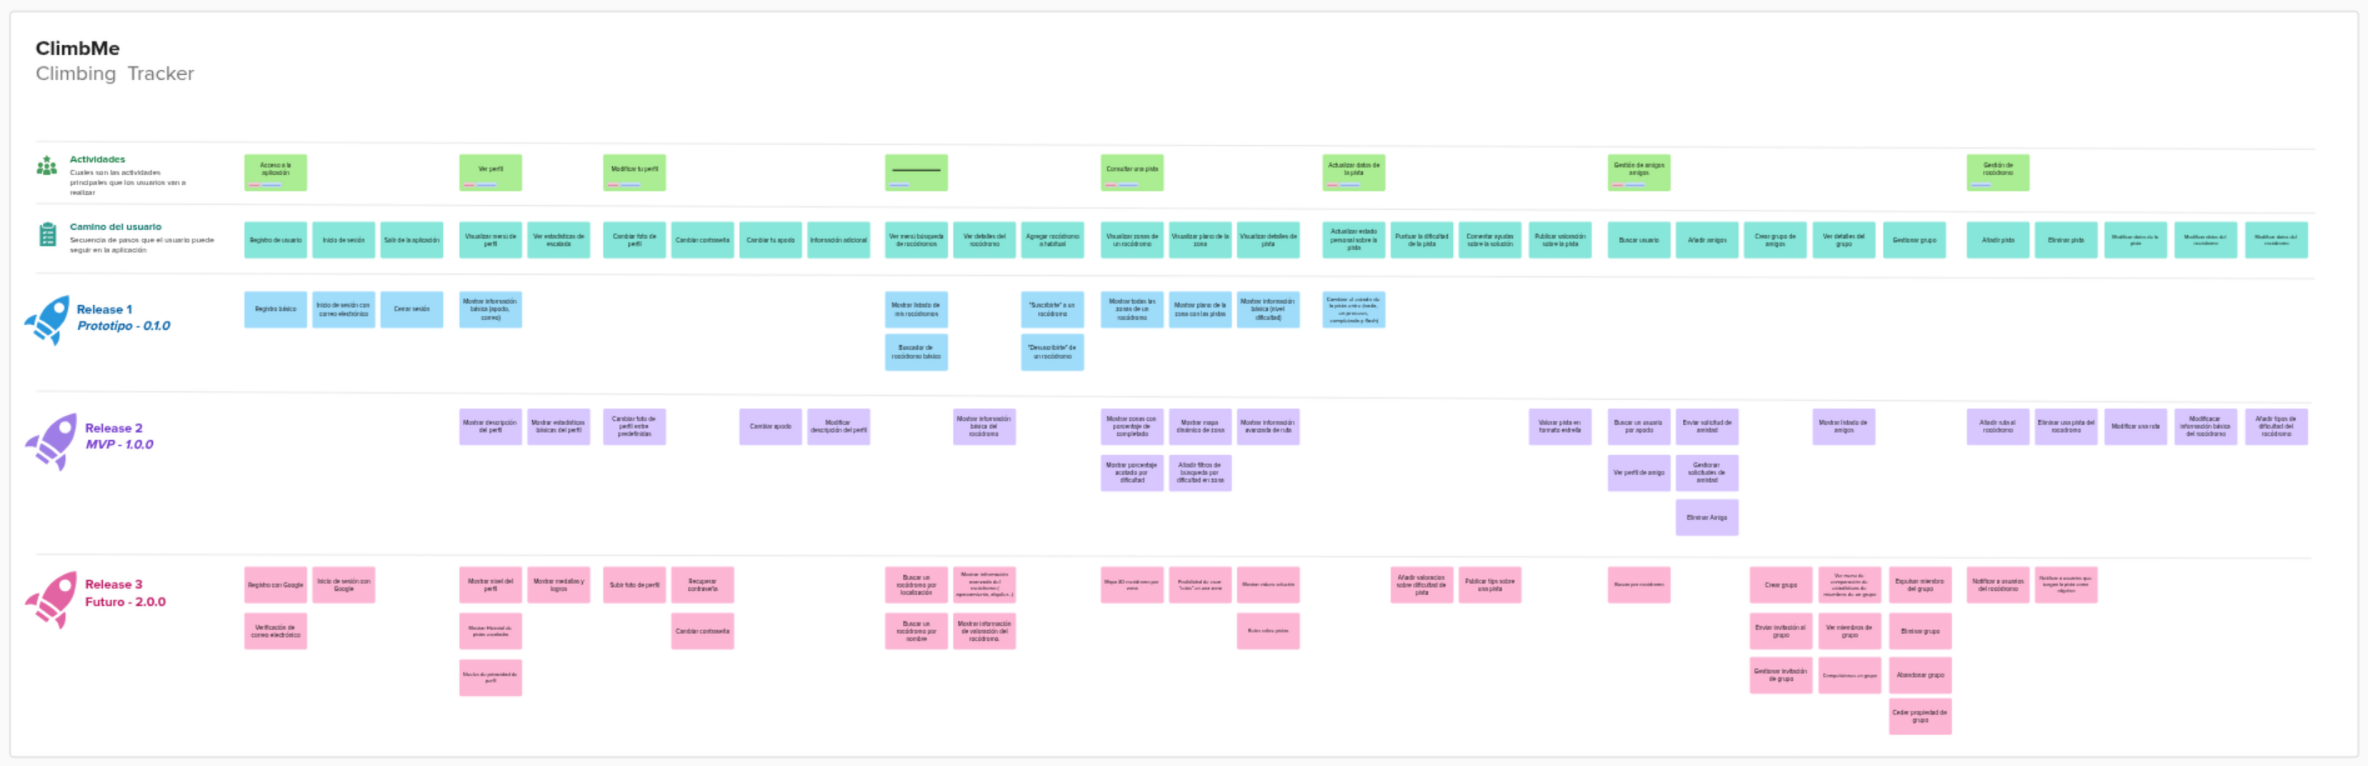
\includegraphics[width=1\textwidth]{./Imagenes/Fuentes/usm_climbit.png} 
    \caption{User Story Map completo de ClimbIt}
    \label{fig:imagen_usm}
\end{figure}


\section{Metodología de trabajo: Scrumban}

Para la gestión del proyecto se optó por la metodología ágil \textbf{Scrumban} \citep{ladas2008scrumban}. Se consideró que aplicar Scrum en estado puro resultaría demasiado estricto y añadiría una carga burocrática excesiva para un equipo de solo dos personas. Por otro lado, el marco de trabajo Kanban carecía de los periodos de desarrollo intensivos y acotados que se necesitaba para este proyecto. Como resultado se empleo Scrumban, una metodología híbrida que combina la flexibilidad basada en flujos de Kanban con la estructura de iteraciones planificadas de Scrum.

De Scrum se heredó el concepto de \textit{sprints} (iteraciones temporales de desarrollo) con una duración de dos semanas y las técnicas de especificación de requisitos mediante Historias de Usuario (HU) y \textit{Epics} (agrupaciones para la definición de casos de uso mayores). Por otro lado, de Kanban se adoptó su sitema de tablero WIP(Work In Progress) como se observa en la imagen \ref{fig:tablero_wip} y el sistema de tracción o \textit{pull} de manera que en lugar de preasignar las tarea durante la planificación, cada miembro del equipo seleccionaba la siguiente tarea a realizar directamente desde la columna \textit{To Do} según el contexto del momento.

\begin{figure}[h]
    \centering
    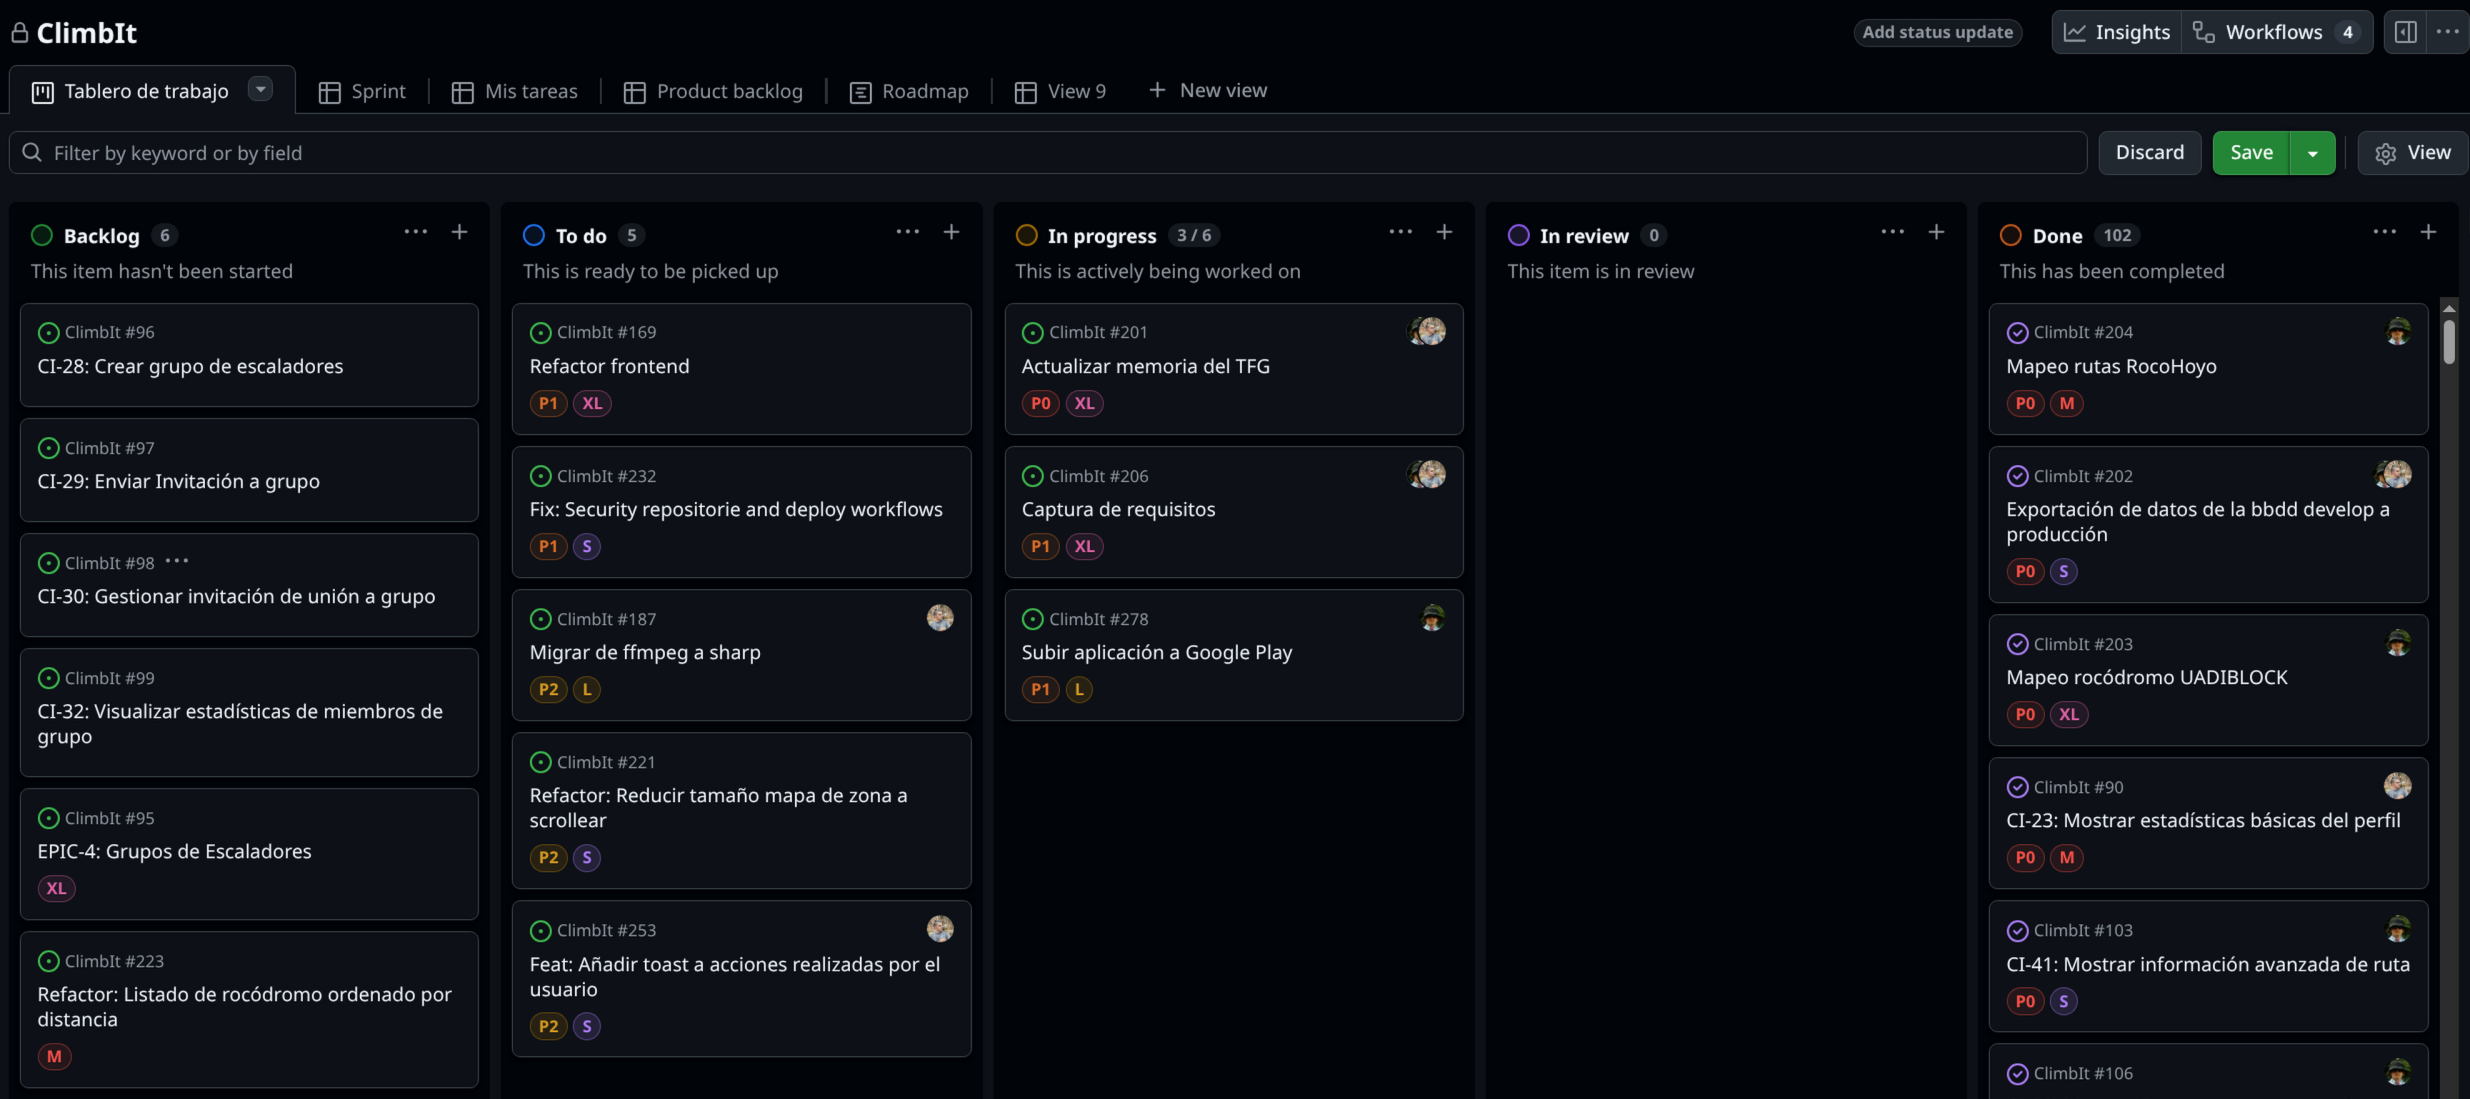
\includegraphics[width=1\textwidth]{./Imagenes/Fuentes/tablero_wip.png} 
    \caption{Tablero WIP de Scrumban implementado en GitHub Projects}
    \label{fig:tablero_wip}
\end{figure}

\section{Herramientas de gestión y seguimiento}

Para la gestión diaria del proyecto, se tomó la decisión de integrar las herramientas de planificación lo más cerca posible del entorno de desarrollo para reducir la fricción al utlizarla. Se descartó el uso de plataformas externas (como Jira o Trello) y se centralizó toda la gestión ágil directamente en \textbf{GitHub Projects}, manteniendo los requisitos estrechamente vinculados al código fuente en \textbf{GitHub Repositories} y al CI/CD en \textbf{GitHub Actions}.

El \textit{Product Backlog} se rellenó progresivamente con las tareas extraídas del \textit{User Story Map} de forma que cada requisito, ya fuera una Historia de Usuario funcional o una tarea técnica o externa, se tradujo en una \textit{Issue} dentro del repositorio con la iformación de la Tabla \ref{tab:config_issues} para no perder contexto.

\begin{table}[h]
\centering
\begin{tabular}{|l|p{10cm}|}
\hline
\textbf{Atributo} & \textbf{Descripción y uso en el proyecto} \\ \hline
\textbf{Título} & Titulo de la tarea o Historia de Usuario. \\ \hline
\textbf{Descripción} & Descripción de la tarea a realizar (Si es HU mediante definición y criterios de aceptación). \\ \hline
\textbf{Estado} & Columna del tablero Kanban (\textit{Backlog, To Do, In Progress, Review, Done}). \\ \hline
\textbf{Labels} & Categorización visual (\textit{bug, backend, frontend, documentación, epic, HU...}). \\ \hline
\textbf{Estimación} & Tamaño (\textit{Size}) desde XS hasta XL para medir el esfuerzo relativo. \\ \hline
\textbf{Prioridad} & Nivel de urgencia (\textit{P0, P1, P2}), marcando P0 las tareas críticas de bloqueo. \\ \hline
\textbf{Milestone} & Vinculación directa al \textit{sprint} actual para seguimiento temporal. \\ \hline
\textbf{Asignados} & Responsables del desarrollo de la tarea \\ \hline
\end{tabular}
\caption{Configuración de una \textit{Issue} en GitHub Projects.}
\label{tab:config_issues}
\end{table}

El seguimiento de los sucesivos \textit{sprints} se apoyó en un \textit{Roadmap} visual como se observa en la imagen \ref{fig:road_map}y en gráficos de evolución del sprint (\textit{Burndown charts}) como el que se aprecia en la imagen \ref{fig:burdown_chart}, permitiendo visualizar de manera cuantitativa el progreso real frente al esperado y detectar si la capacidad de desarrollo había sido sobrestimada.

\begin{figure}[h]
    \centering
    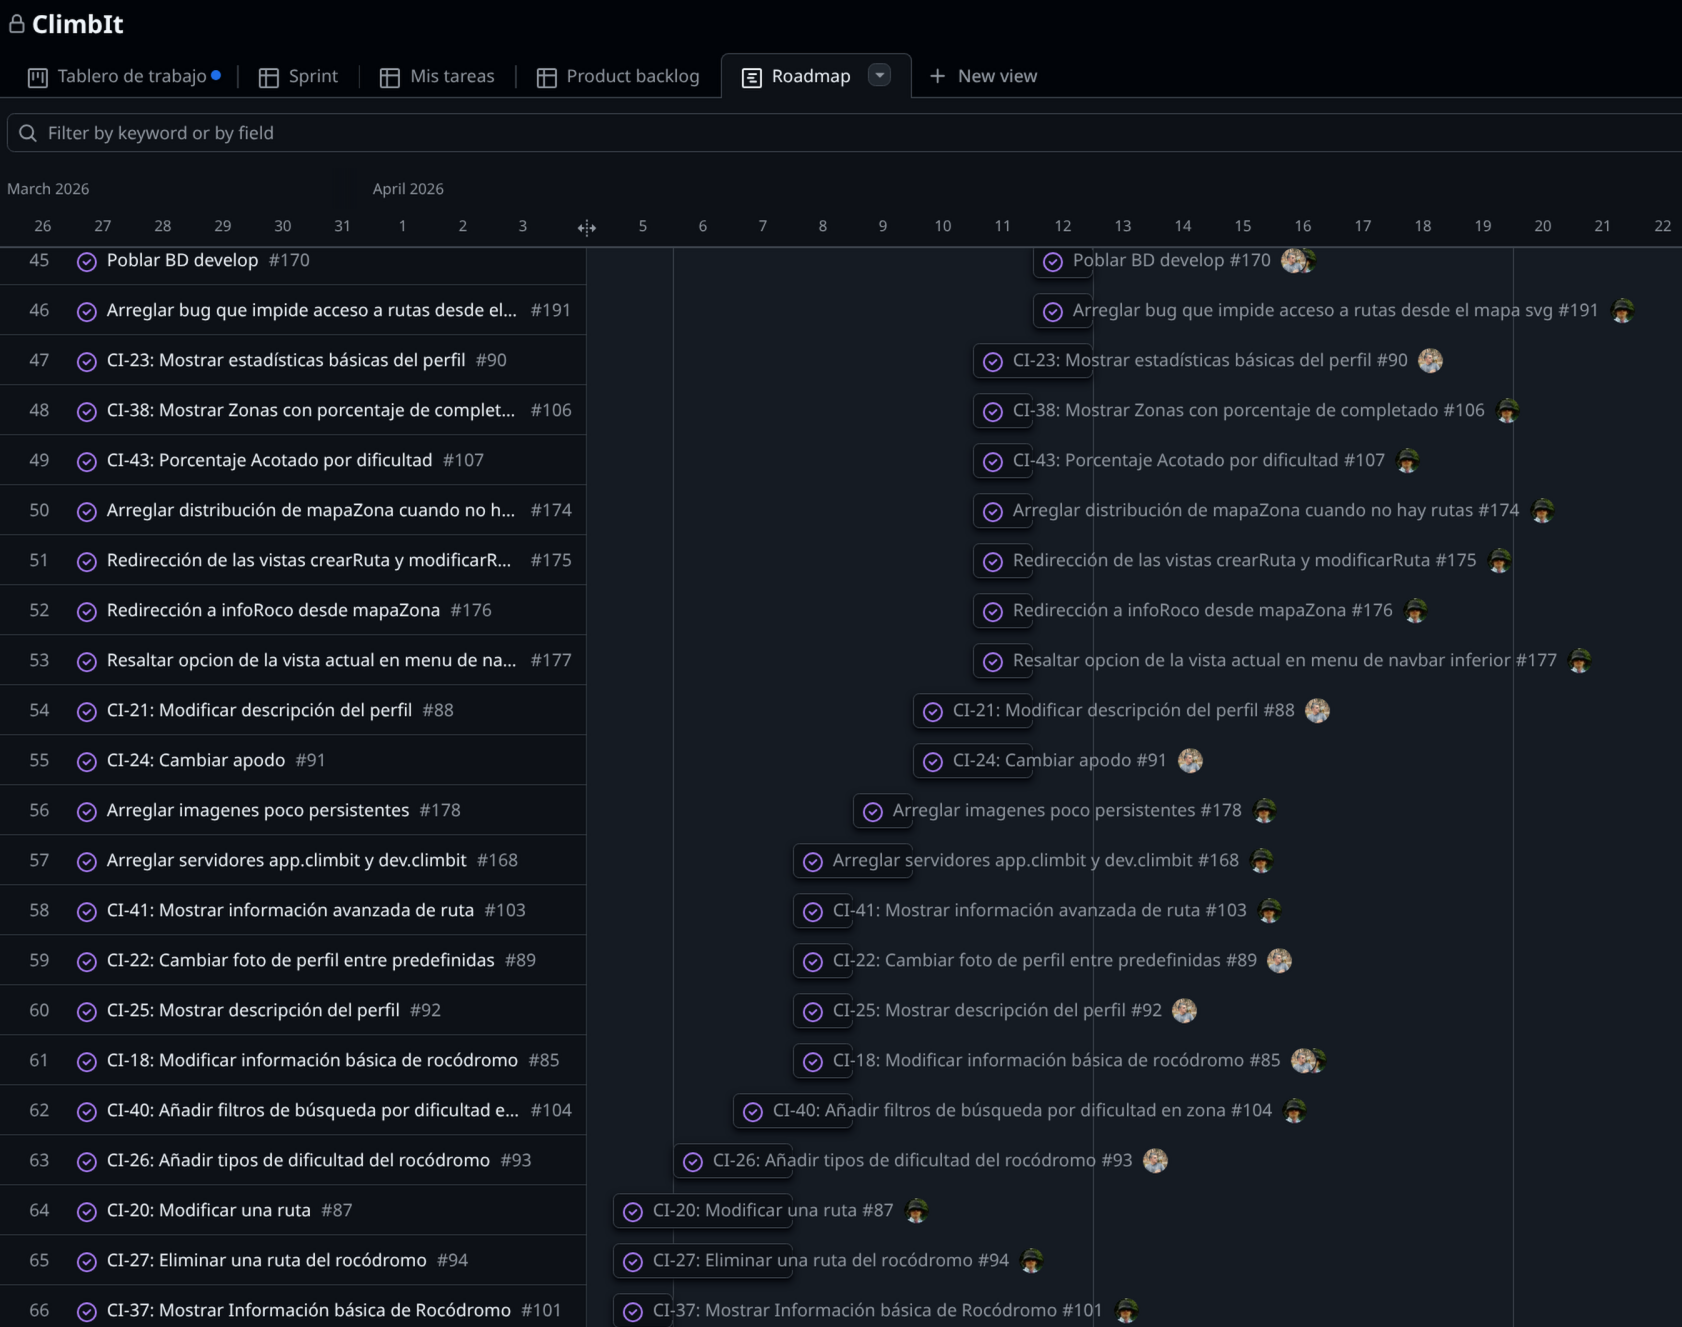
\includegraphics[width=1\textwidth]{./Imagenes/Fuentes/roadmap_github.png} 
    \caption{Roadmap implementado con GitHub Projects}
    \label{fig:road_map}
\end{figure}

\begin{figure}[h]
    \centering
    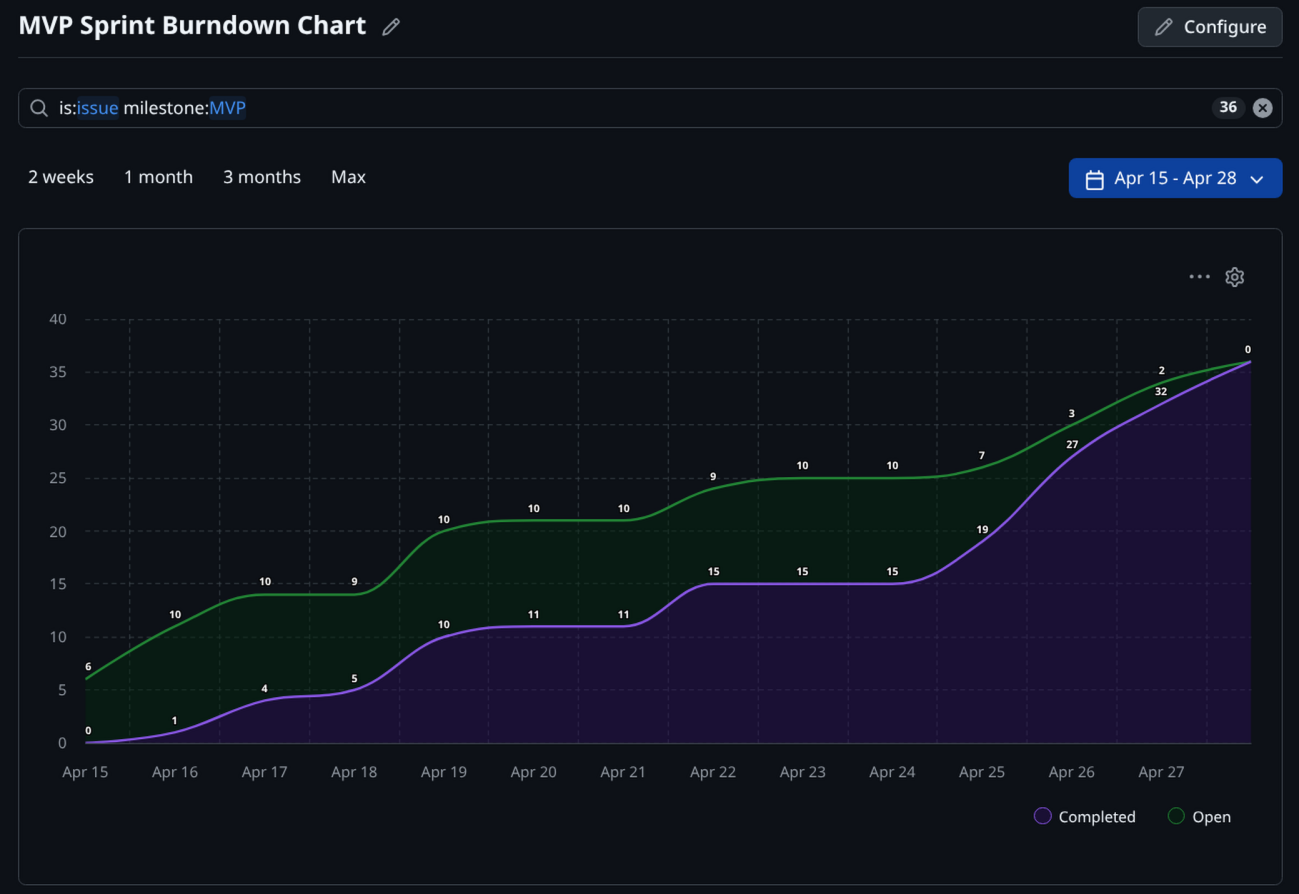
\includegraphics[width=0.8\textwidth]{./Imagenes/Fuentes/burdownChart_mvp.png} 
    \caption{Burndown chart del cuarto sprint realizado}
    \label{fig:burdown_chart}
\end{figure}

\section{Gestión de la Configuración y Control de Versiones}

Se implementó un flujo de trabajo basado en el estándar \textbf{Git Flow}, estableciendo reglas estrictas sobre cómo integrar el código de cada desarrollador. En el repositorio existieron dos ramas principales protegidas: la rama \texttt{main} se reservó exclusivamente para las versiones estables y liberadas del producto (las cuales se volcaban a producción), mientras que \texttt{develop} actuaba como el entorno de integración constante para los nuevos casos de uso.

Cada \textit{Issue} del tablero requería la creación de una rama específica de funcionalidad (\textit{feature branch}). Al finalizar el desarrollo, esta rama se integraba en \texttt{develop} a través de \textit{Pull Requests} revisadas bajo una estrategia de \textit{squash and merge}. Esto permitió agrupar decenas de pequeños \textit{commits} locales en un solo bloque semántico consolidado, manteniendo un historial limpio y coherente.

En paralelo, el despliegue se gestionó mediante la herramienta de \textit{Releases} de GitHub. Se adoptó el versionado semántico clásico (X.Y.Z) y se mantuvo la trazabilidad técnica de los cambios a través de un archivo \texttt{CHANGELOG.md} basado en el estándar \textit{Keep a Changelog}. A nivel organizativo, el repositorio se dotó desde el inicio con archivos \texttt{.gitignore} apropiados para el \textit{stack} tecnológico y una completa guía de instalación en el \texttt{README.md}.

\section{Uso de Inteligencia Artificial como Apoyo al Desarrollo}

Durante el ciclo de vida del proyecto, se han empleado herramientas de Inteligencia Artificial (IA) generativa como asistentes de desarrollo. La principal justificación para su uso ha sido la reducción de tiempos en la codificación de componentes rutinarios y la aceleración en la investigación de nuevas tecnologíascon el objetivo de lograr cumplir con el objetivo del Diseño Centrado en el Usuario de llegar a realizar varias iteraciones de testeo y validación con usuarios finales reales, algo que difícilmente se habría conseguído lograr con el alcance establecido en los plazos académicos dados.

El uso de esta tecnología no sustituyó en ningún momento la toma de decisiones, el diseño de la arquitectura general ni la lógica de negocio. Su integración en el flujo de trabajo se estructuró en dos grandes bloques:

\paragraph{Investigación y adopción de buenas prácticas:} En las fases de exploración técnica, la IA se empleo como una herramienta informativa para mejorar y acelerar nuestra toma de decisiones. Por ejemplo, a la hora de implentar un mapa dinámico como el de la herramienta TopLogger se consulto para ver las librerías existentes, o de igual forma, se utilizó para consultar los pasos ha seguir para subir una aplicación PWA a Google Play. Esto nos permitió filtrar grandes volúmenes de documentación oficial eficientemente y fundamentar una toma de decisiones más informada.

\paragraph{Automatización de tareas repetitivas y reducción de carga cognitiva:} Durante la implementación, en fases de creación de código repetitivo que no aportan valor innovador nuestra política de desarrollo con IA consistió en que, una vez que la arquitectura y el diseño habían sido definidos, analizados y programados manualmente al menos una vez por el equipo como por ejemplo, el diseño de tarjetas de las estadísticas, se utilizó la IA para replicar y adaptar esos patrones en otros componentes equivalentes. Al delegar esta repetición mecánica, se logró redirigir la carga de trabajo hacia tareas más críticas. Sobre todo el código generado se realizo una revisión exhaustiva, control de errores y validación.